\documentclass[article]{jss}
\usepackage{amsmath}

\author{David M Diez\\Harvard Biostatistics}
\title{Survival Analysis in \proglang{R}: A Tutorial}

\Plainauthor{David M diez}
\Plaintitle{Survival Analysis in R: A Tutorial} %% without formatting
%\Shorttitle{Survival Analysis in R} %% a short title (if necessary)

\Abstract{
This tutorial introduces the \pkg{survival} package in \proglang{R} to readers with a passing familiar with survival analysis and basic familiarity with objects and plotting in \proglang{R}. This tutorial begins with the basics of building survival objects all the way up through fitting Cox proportional hazards for time-varying covariates.
}
\Keywords{survival analysis, \code{survival} package, \proglang{R}, tutorial, OpenIntro}
\Plainkeywords{survival analysis, survival package, R, tutorial, OpenIntro}

%% publication information
%% NOTE: Typically, this can be left commented and will be filled out by the technical editor
%% \Volume{13}
%% \Issue{9}
%% \Month{September}
%% \Year{2004}
%% \Submitdate{2004-09-29}
%% \Acceptdate{2004-09-29}

\Address{
  David M Diez\\
  Department of Biostatistics\\
  Harvard School of Public Health\\
  655 Huntington Avenue \\
  SPH2, 4th Floor \\
  E-mail: \email{david.m.diez@gmail.com}\\
  URL: \url{http://www.openintro.org/}
}

\begin{document}

%% Note that you should use the \pkg{}, \proglang{} and \code{} commands.

\section[Introduction]{Introduction}

Survival analysis is the study of time-to-event data. This document is intended to assist individuals knowledgable in the basics of survival analysis and interested in applying survival analysis in \proglang{R} with the \pkg{survival} package \citep{survival}. Familiarity with data objects, plotting, and linear models in \proglang{R} is assumed. The reader who plans to print this document will find reading easiest if this paper is printed front-to-back and bound like a book. Under this construction, topics running two pages will be fully visible without the turn of a page.

Each section introduces a new set of survival analysis tools in \proglang{R}, and these topics are introduced in the following order. The \pkg{survival}, \pkg{OIsurv}, and \pkg{KMsurv} packages are introduced in Section~\ref{packagesAndData}. Methods for constructing survival objects are introduced in Section~\ref{survObjects}. The nonparametric Kaplan-Meier estimate of the survival curve, its pointwise bounds, and confidence bands are introduced in Sections~\ref{kapMeiEstimateAndBounds} and~\ref{confBands}. Section~\ref{cumulativeHazard} introduces the cumulative hazard function. Estimation of the mean, median, and their corresponding confidence intervals are described in Section~\ref{meanAndMedianEstimates}. Techniques for conducting simple tests on survival data are introduced in Section~\ref{testsForTwoOrMoreSamples}. Sections~\ref{coxPHConstCov} and~\ref{coxPHTimeDepCov} introduce methods for fitting Cox proportional hazards models when covariates are constant and time-varying, respectively. Accelerated failure-time models are outlined and discussed in Section~\ref{accFailureTimeModels}.

\pagebreak

\section[Three packages]{Three packages: \pkg{survival}, \pkg{OIsurv}, and \pkg{KMsurv}}
\label{packagesAndData}

Methods and data sets from the \pkg{survival}, \pkg{OIsurv}, and \pkg{KMsurv} packages in \proglang{R} are utilized throughout this document \citep{survival, OIsurv, KMsurv}. The \pkg{survival} package is a plentiful supply of survival analysis functions and is one of the packages that comes with a standard \proglang{R} installation. The \pkg{OIsurv} and \pkg{KMsurv} packages offer supplemental functions and data. Both packages can be installed through the \code{install.packages} function. Installing \pkg{OIsurv} will install both packages.
\begin{verbatim}
> install.packages('OIsurv')
\end{verbatim}
%The \pkg{OIsurv} package depends on the \pkg{KMsurv} package, so the first automatically installs the second (if necessary). 
Similarly, loading the \pkg{OIsurv} package using the \code{library} function will load other dependent packages, including \pkg{survival} and \pkg{KMsurv}.
\begin{verbatim}
> library(OIsurv)  # the survival package depends on the splines package
Loading required package: survival
Loading required package: splines
Loading required package: KMsurv
\end{verbatim}
To view available data sets in the \pkg{KMsurv} package, use \code{library(help=KMsurv)}; these data sets are featured in \citet{Klein2003}. To load a data set, use the \code{data} function, and to view the help file of a data set or function, use the \code{?} command:
\begin{verbatim}
> data(aids)
> aids
    infect induct adult
1     0.00   5.00     1
...
295   7.25   0.25     0
> ?aids    # opens help document for aids data set
> ?OIsurv  # OIsurv's help file examples include all code in this tutorial
\end{verbatim}
%294   7.00   0.75     0
The '\code{...}' denotes output omitted for brevity. The code of any individual section of this tutorial may be run when the \pkg{survival}, \pkg{OIsurv}, and \pkg{KMsurv} packages are loaded into an \proglang{R} session.

For brevity in code, this document will make columns from a data frame accessible as free-standing variables via the \code{attach} function.
\begin{verbatim}
> attach(aids)
> infect
  [1] 0.00 0.25 0.75 0.75 0.75 1.00 1.00 1.00 1.00 1.25 1.25 1.25 1.25 1.50
...
[295] 7.25
\end{verbatim}
%The variable \code{infect} is associated with the \code{aids} data set. For this reason, it is more common for R users to access a variable from a data set via the \code{\$} operator:
%\begin{verbatim}
%> aids$infect
%...
%\end{verbatim}
Detaching the data set after the analysis can prevent errors, as some data frames share column (variable) names.
\begin{verbatim}
> detach(aids)
\end{verbatim}
Unless otherwise noted, functions and data sets introduced and used in this tutorial come from the \pkg{survival} and \pkg{KMsurv} packages, respectively.

\pagebreak



\section[Survival objects]{Survival objects} %: \code{Surv(time, event, time2, type)}}
\label{survObjects}

Many functions in the \pkg{survival} package apply methods to objects (variables) of class \code{"Surv"}. The \code{Surv} function is used to put data into this proper format. Here we discuss how to construct right-censored, left-censored, and interval censored objects of class \code{"Surv"}. For a review of these data types, see~\citet{formsOfSurvData} or~\citet{Klein2003}. The \code{Surv} function has four commonly used arguments: \code{time}, \code{time2}, \code{event}, and \code{type}.

\textbf{Right-censored} data occur when each case is tracked and either the event time is known and observed, or it has not occurred up to some time where observation is ended. Formatting right-censored data using \code{Surv} requires only two arguments. The first argument represents the time and the second is an indicator specifying whether the time is for an event (\code{1}) or a right-censored (\code{1}) observation.
\begin{verbatim}
> data(tongue)
> attach(tongue)
> mySurvObject <- Surv(time, delta)
> mySurvObject
 [1]   1    3    3    4   10   13   13   16   16   24   26   27 
...
[73] 129  181    8+  67+  76+ 104+ 176+ 231+
> detach(tongue)
\end{verbatim}
The '\code{+}' symbol is used to signify right-censoring. 
%An indicator vector is used in the \code{event} argument to signify whether the event was censored (\code{1}) or not (\code{0}). Boolean arguments may be used in place of \code{1} and \code{0} in the \code{event} argument.

\textbf{Left-censoring} occurs when the event is known to have occurred before some time. For these data, the \code{time}, \code{event}, and \code{type} arguments are used to specify \textbf{left-censoring} in the \code{Surv} function. The first two arguments are identical to those for right-censoring, and the \code{type} argument must be specified as \code{"left"}:
\begin{verbatim}
> # Surv(time, event, type="left")
\end{verbatim}

\textbf{Interval-censoring} occurs when the event is known to lie in some interval. Here we introduce one technique for creating interval-censored data that will be applied in Section~\ref{coxPHTimeDepCov} for time-dependent covariates. Suppose we encounter two types of individuals:
\begin{enumerate}
\item those who have an event between two times, where those times may be distinct for each individual, and
\item individuals who are observed for an interval of time but the event is not observed, i.e. these observations are right-censored.
\end{enumerate}
Then we might summarize the intervals for these two groups as $(t_1, t_2]$ and $(t_1, t_2]+$, respectively. We can construct such data in \proglang{R} by specifying the $t_1$ and $t_2$ times as \code{time} and \code{time2}, and also specifying the event argument:
\begin{verbatim}
> # Surv(t1, t2, event)
\end{verbatim}
In this code, \code{t1} and \code{t2} are vectors representing $t_1$ and $t_2$.

%The second construction of intervals uses the \code{time}, \code{time2}, and \code{type} arguments. Here data is considered where observations might fall into four categories: exact, right-censored, left-censored, or both interval-censored (both left and right-censored). The trick is to use \code{NA} to specify -$\infty$ and +$\infty$. For instance, we construct observations of all four types below, respectively:
%\begin{verbatim}
%> t1 <- c(NA, 3, 3, 3)
%> t2 <- c(3, NA, 5, 3)
%> Surv(t1, t2, type="interval2")
%[1] 3-     3+     [3, 5] 3
%\end{verbatim}
%The exact time is specified using an interval that is equal to a point in time.

There are additional ways to construct survival data, which are described in the help file for the \code{Surv} function. For instance, a second type of interval censoring can be accomplished using \code{type="interval"}.

%To do interval censoring, use \code{time} for the intervals' left ends, \code{time2} for the intervals' right ends, and set \code{type="interval2"}. The \code{event} argument again indicates whether the event was observed or right-censored. There are more types of survival data that may be transformed into a survival object, however, they will not be discussed here. % {\color{red} Verify the following:} Note that not all functions will accept all types of data. For example, interval-censored data will not be accepted by many of the functions in \pkg{survival}.

\pagebreak

%%% KAPLAN - MEIER %%%
\section[Kaplan-Meier estimate and pointwise bounds]{Kaplan-Meier estimate and pointwise bounds}
\label{kapMeiEstimateAndBounds}

The Kaplan-Meier estimate is a nonparametric maximum likelihood estimate (MLE) of the survival function, $S(t) = P(T > t)$. The estimate is a step function with jumps at observed event times, $t_i$. The description below assumes the $t_i$ are ordered: $0 < t_1 < t_2 <  \cdots < t_D$. If the number of individuals with an observed event time $t_i$ is $d_i$, and $Y_i$ is the number of individuals at risk -- i.e.\hspace{1mm}no event has occurred for these cases -- at a time before $t_i$, then the Kaplan-Meier estimate of the survival function and its estimated variance is given by
\begin{eqnarray*}
\hat{S}(t) &=& \left\{\begin{array}{cl}1 & \text{if }t < t_1 \\ \prod_{t_i \leq t}\left[ 1- \frac{d_i}{Y_i} \right] &\text{if }t_1 \leq t \end{array}\right.  \\
\widehat{V}[\hat{S}(t)] &=& \left[ \hat{S}(t) \right]^2 \hat{\sigma}_S^2(t) = \left[ \hat{S}(t) \right]^2 \sum_{t_i \leq t} \frac{d_i}{Y_i(Y_i-d_i)}
\end{eqnarray*}
One estimate of the pointwise confidence bounds %for a %\code{"plain"} (
%linear %) %and \code{"log-log"} options
%option %provided in \pkg{survival} are 
is given by
\begin{eqnarray} \label{plainPWCI}
\hat{S} \pm Z_{1-\alpha/2}\hat{\sigma}_S(t)\hat{S}(t)
%\left( \hat{S} - Z_{1-\alpha/2}\hat{\sigma}_S(t)\hat{S}(t), \ \hat{S} + Z_{1-\alpha/2}\hat{\sigma}_S(t)\hat{S}(t) \right) \\
%\left(\hat{S}^{1/\theta}(t), \ \hat{S}^\theta(t)\right)\text{, where }\theta = \exp\left\{ \frac{Z_{1-\alpha/2}\hat{\sigma}_S(t)}{\log \hat{S}(t) } \right\}
\end{eqnarray}

The Kaplan-Meier estimate is fit in \proglang{R} using the function \code{survfit} function from the \pkg{survival} package. The only required argument is a formula where the survival object is the response. To fit the estimated survival curve of a set of data, the survival object is regressed against \code{1}:
\begin{verbatim}
> data(tongue)
> attach(tongue)
> mySurv <- Surv(time[type==1], delta[type==1])
> (myFit <- survfit(mySurv ~ 1))
Call: survfit(formula = mySurv ~ 1)

records   n.max n.start  events  median 0.95LCL 0.95UCL 
     52      52      52      31      93      67      NA 
\end{verbatim}
The confidence level may be changed using an argument called \code{conf.int} (e.g. \code{conf.int=0.90} for 90\% confidence bounds). The \code{conf.type} argument describes the type of confidence interval. More specifically, it describes the transformation for constructing the confidence interval. The default is \code{'log'}, which equates to the transformation function $g(t) = \log(t)$. The \code{'log-log'} option uses $g(t) = \log(-\log(t))$. A linear confidence interval fitting the description of Equation~\eqref{plainPWCI} is created using the \code{conf.type='plain'} option. At this time, the arcsine-squareroot transformation is not an available option, but it can be computed manually using the elements of the summary of an object returned by \code{survfit}.



% There are three arguments of particular interest: \code{formula}, \code{conf.int}, and \code{conf.type}. \code{formula} will be a survival object (and can be made more complex), and it is the only required input:

%The argument \code{conf.int} is the confidence interval level and ranges between \code{0} and \code{1} with the default \code{0.95}. \code{conf.type} is the type of confidence interval or, more accurately, the transformation used to construct the confidence interval. The default is \code{'log'}, which equates to the transformation function $g(t) = \log(t)$, \textbf{not} $g(t) = \log(-\log(t))$, which is \code{'log-log'}. A linear confidence interval is created by using the argument \code{conf.type='plain'}.

Like the \code{lm} function in \proglang{R}, we can generate a summary of the output of \code{survfit}.
\begin{verbatim}
> summary(myFit)
Call: survfit(formula = mySurv ~ 1)

 time n.risk n.event survival std.err lower 95% CI upper 95% CI
    1     52       1    0.981  0.0190        0.944        1.000
    3     51       2    0.942  0.0323        0.881        1.000
...
  167      4       1    0.229  0.0954        0.101        0.518
\end{verbatim}
Also just like \code{lm}, the output of \code{survfit} is a list, and each item in the list may be accessed using the \code{$} operator. We consider many of these elements below; the actual output of each is hidden for brevity.
\begin{verbatim}
> myFit$surv     # outputs the Kaplan-Meier estimate at each t_i
> myFit$time     # {t_i}
> myFit$n.risk   # {Y_i}
> myFit$n.event  # {d_i}
> myFit$std.err  # standard error of the K-M estimate at {t_i}
> myFit$lower    # lower pointwise estimates (alternatively, $upper)
\end{verbatim}
%All available items may be listed via the \code{str} command: \code{str(myFit)}.

%The simple commands above would yield a survival function fit, which may be obtained either by looking at \code{summary(survfit(my.surv ~ 1))} or by looking at the function's hidden output. This hidden information is where the Kaplan-Meier estimate, a 95\% confidence bound, along with the $\{t_i\}$, $\{d_i\}$, and $\{Y_i\}$ are saved. All of this data will be output by looking at the summary. To get the output in individual vectors, use the following commands (the actual outputs are omitted for brevity):
%\begin{verbatim}
%> my.fit <- survfit(my.surv)
%> summary(my.fit)$surv     # outputs the Kaplan-Meier estimate at each t_i
%> summary(my.fit)$time     # {t_i}
%> summary(my.fit)$n.risk   # {Y_i}
%> summary(my.fit)$n.event  # {d_i}
%> summary(my.fit)$std.err  # standard error of the K-M estimate at {t_i}
%> summary(my.fit)$lower    # lower pointwise estimates (alternatively, $upper)
%\end{verbatim}
The \code{plot} method may also be applied to the Kaplan-Meier estimate from the \code{surv.fit} function, as shown in Figure~\ref{kmPlot}. The familiar arguments in the plot function may be used to improve the graphical aesthetics:
\begin{verbatim}
> plot(myFit, main="Kaplan-Meier estimate with 95% confidence bounds",
+      xlab="time", ylab="survival function")
\end{verbatim}
\begin{figure}
\centering
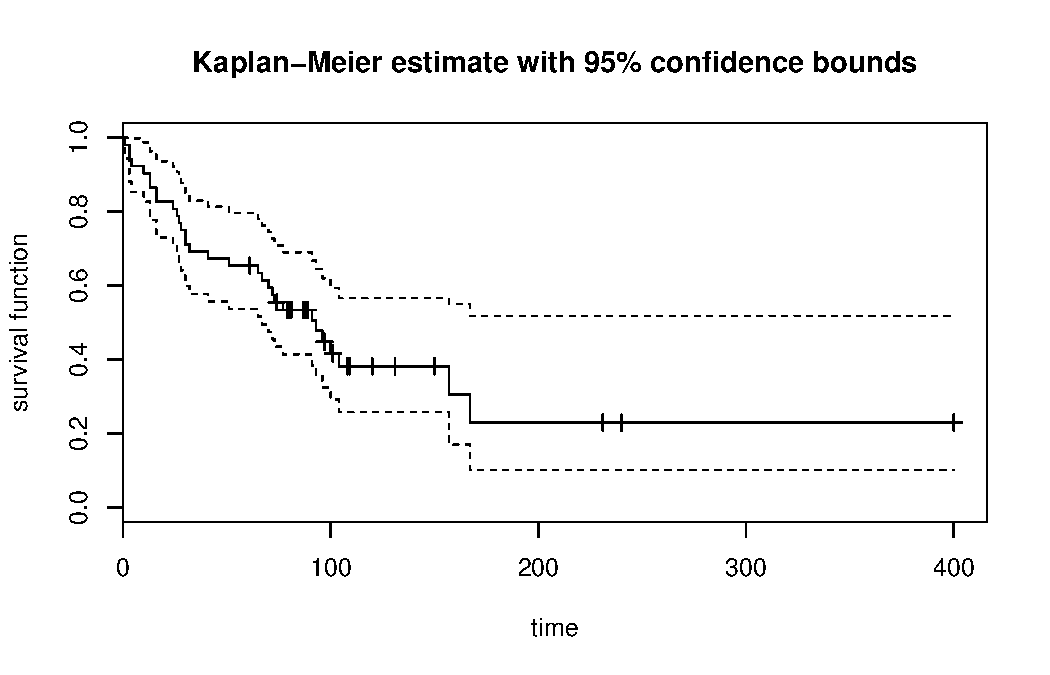
\includegraphics[width=0.7\textwidth]{../../figures/kmPlot.pdf}
\caption{Sample output of \code{plot(myFit, ...)}, where the title, x-axis and y-axis labels have been specified via the \code{main}, \code{xlab}, and \code{ylab} arguments, respectively.}
\label{kmPlot}
\end{figure}
Sometimes different groups are mixed together in a single \code{Surv} object. If a separate vector specifies which cases correspond to which groups, then these groups can be separated by regressing the \code{Surv} object on that vector:
\begin{verbatim}
> myFit1 <- survfit(Surv(time, delta) ~ type)  # 'type' specifies the grouping
\end{verbatim}
The list output by the summary of \code{myFit1} will contain an additional list item called \code{strata} -- accessible via \code{summary(myFit1)$strata} -- which designates which components of the output correspond to which groups.

Finally, for good coding practices, we detach the \code{tongue} data set.
\begin{verbatim}
> detach(tongue)
\end{verbatim}

%\textbf{Other options:} The \code{type} argument offers alternative estimates. The default is the Kaplan-Meier estimate (\code{'kaplan-meier'}) while other options are \code{'fleming-harrington'} and \code{'fh2'}. 


\pagebreak

%%% Confidence Bands %%%
\section[Confidence bands]{Kaplan-Meier confidence bands}
%\section{\code{conf.bands(x, conf.type='plain', type='ep', tL=NA, tU=NA)}}
\label{confBands}

The confidence interval bands constructed on the previous pages are only pointwise confidence intervals. General confidence bands can also be constructed using the \code{confBands} function from the \pkg{OIsurv} package. These bands provide bounds on an entire range of time. %That is, a part of the true survival curve crosses outside of a 95\% confidence band in about 5\% of all such cases.

We start by constructing the regular confidence interval bands, just as did in the last section:
\begin{verbatim}
> data(tongue)
> attach(tongue)
> mySurv <- Surv(time[type==1], delta[type==1])
> plot(survfit(mySurv ~ 1), xlab='time',
+      ylab='Estimated Survival Function',
+      main='Confidence intervals versus confidence bands')
\end{verbatim}
Next the \code{confBands} function is used to generate an object of class \code{"confBands"}, which is a list of three items: \code{time}, \code{lower}, and \code{upper}. These values describe the confidence bands, and they are impacted by a number of options within the \code{confBands} function. The only required element of the function is a survival object.
\begin{verbatim}
> myCB <- confBands(mySurv)
> lines(myCB, lty=3)
> legend('topright', legend=c('K-M survival estimate',
+      'pointwise intervals','EP confidence bands'), lty=1:3)
> detach(tongue)
\end{verbatim}
Users may opt to specify more precise types of confidence bands. For instance, the confidence bands can be constructed using different transformations using the \code{confType} argument, or a different confidence level may be specified with \code{confLevel}. These additional options and others are described in the \code{confBands} help file.
\begin{figure}[hb]
\centering
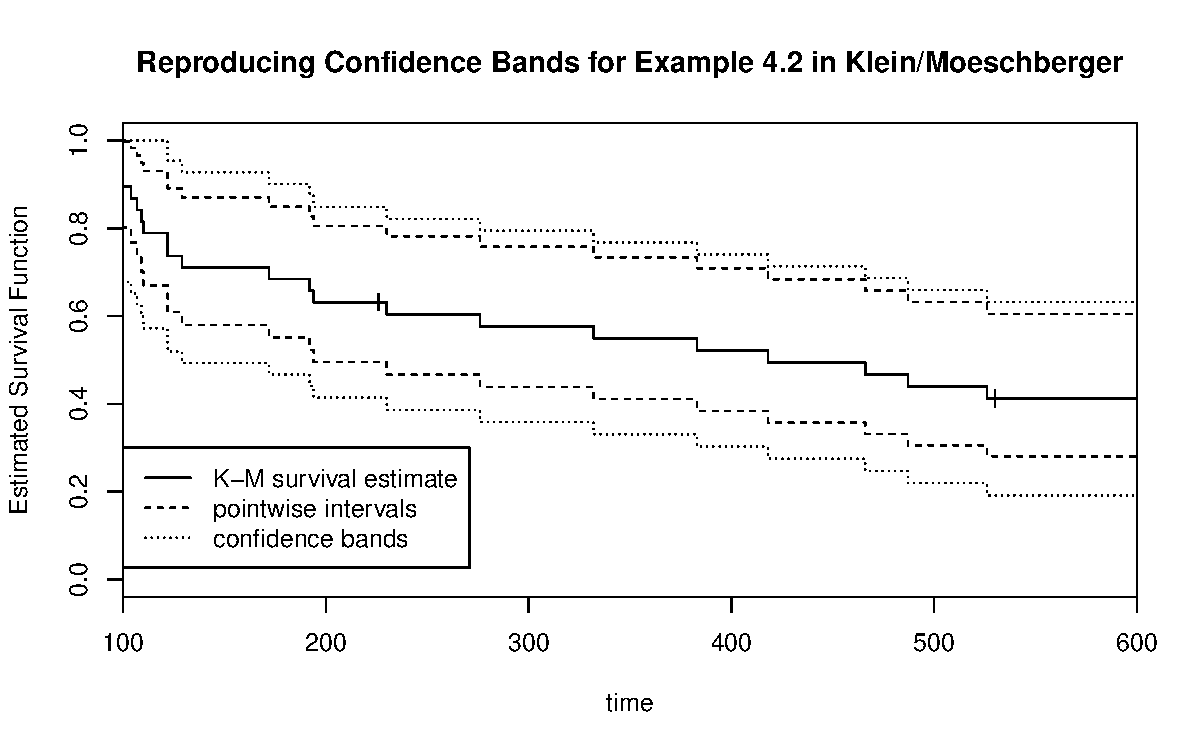
\includegraphics[width=0.73\textwidth]{../../figures/confBand.pdf} \vspace{-4mm}
\caption{Confidence intervals and bans. The default for the pointwise confidence bands is a log transformation, which results in non-symmetric pointwise confidence intervals.} % {\footnotesize\color{red}KM Ex 4.2!}}
\label{confBand}
\end{figure}

\pagebreak

%%% Cumulative Hazard %%%
\section[Cumulative hazard]{Cumulative hazard}
\label{cumulativeHazard}

The relationship between the cumulative hazard function and the survival function is shown in the left side of Equation~\eqref{kmToCumHaz}. Thus, the MLE estimate of the cumulative hazard function may be estimated by transforming the Kaplan-Meier estimate:
\begin{align}\label{kmToCumHaz}
S(t) &= \exp\left\{-H(t)\right\}
&\hat{H}(t) &= -\log\hat{S}(t)
\end{align}
%The MLE of the hazard function may be obtained by transforming the Kaplan-Meier estimate: $$.
Another method to estimate $H(t)$ is the Nelson-Aalen estimator:
\begin{align*}
\widetilde{H}(t) &= \sum_{t_i \leq t} \frac{d_i}{Y_i}\text{ (assuming }t_1\leq t\text{, otherwise it is 0), }
		\qquad \hat{\sigma}_{\widetilde{H}}^2(t) = \sum_{t_i\leq t}\frac{d_i}{Y_i^2}
\end{align*}
No function in the \pkg{survival} package computes either form of the cumulative hazard function, but this can be accomplished using output from \texttt{survfit()}:
\begin{verbatim}
> data(baboon)
> attach(baboon)
> mySurv  <- Surv(time, observed)
> myFit   <- summary(survfit(mySurv ~ 1))
> Hhat    <- -log(c(myFit$surv, tail(myFit$surv, 1)))
\end{verbatim}
A plot of both the MLE and Nelson-Aalen curves may also be constructed:
\begin{verbatim}
> hSortOf <- myFit$n.event / myFit$n.risk
> Htilde  <- c(cumsum(hSortOf), sum(hSortOf))
> plot(c(myFit$time, 1200), Hhat, xlab='time', ylab='cumulative hazard',
+      main='Comparing cumulative hazards', type='s')
> lines(c(myFit$time, 1200), Htilde, lty=2, type='s')
> legend('topleft', legend=c('MLE', 'Nelson-Aalen'), lty=1:2)
> detach(baboon)
\end{verbatim}
\begin{figure}[htp]
\centering
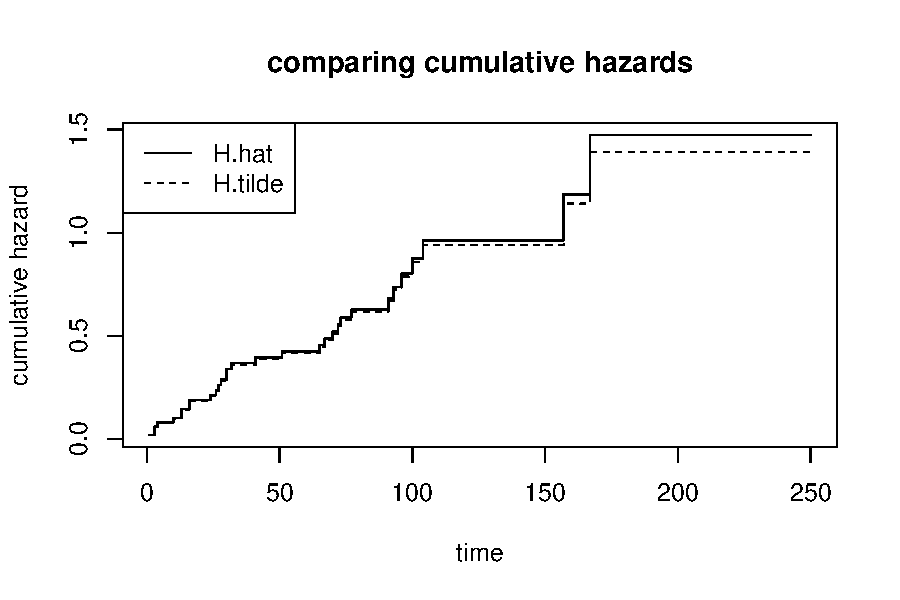
\includegraphics[width=0.72\textwidth]{../../figures/cumHazard}
\caption{Estimates of the cumulative hazard function via MLE and Nelson-Aalen methods.}
\label{cumHazard}
\end{figure}

\pagebreak

%%% Compute mean and median estimates %%%
\section[Mean and median estimates with bounds]{Mean and median estimates with bounds}
\label{meanAndMedianEstimates}

The median survival time is the time $t_{0.5}$ such that $S(t_{0.5}) = 0.5$, visualized by graphing the survival function estimate, drawing a horizontal line at 0.5, and identifying the time at which the survival curve and line intersect. The confidence bounds for $t_{0.5}$ are given by the points at which this horizontal line crosses over the confidence bounds of $\hat{S}(t)$. The median and its bounds may be estimated using the \texttt{survfit} function:
\begin{verbatim}
> data(drug6mp)
> attach(drug6mp)
> mySurv <- Surv(t1, rep(1, 21))   # all placebo patients observed
> survfit(mySurv ~ 1)
Call: survfit(formula = mySurv ~ 1)

records   n.max n.start  events  median 0.95LCL 0.95UCL 
     21      21      21      21       8       4      12 
\end{verbatim}

\noindent The mean survival time and its respective estimate are given by
\begin{align*}
\mu &= \int_0^\infty S(t)dt
	&\hat{\mu} &= \int_0^\infty \hat{S}(t)dt
\end{align*}
If $S(t)$ (or $\hat{S}(t)$) does not converge to zero, the integral diverges. To avert this disaster, it is common to use a finite value $\tau$ as the bound for the integral, creating a biased estimate of the mean, shown in the left side of Equation~\eqref{truncatedMean}. For instance, one might choose $\tau$ as the largest observed or censored time. Using the values $t_i$, $Y_i$, $d_i$, and $D$ defined in Section~\ref{kapMeiEstimateAndBounds}, the estimated variance of $\hat{\mu}_\tau$ is given in the right side of Equation~\eqref{truncatedMean}.
\begin{align} \label{truncatedMean}
\mu_\tau &= \int_0^\tau S(t)dt 
&\hat{V}(\hat{\mu}_\tau) &= \sum_{i=1}^D\left[\int_{t_i}^\tau \hat{S}(t)dt\right]^2 \frac{d_i}{Y_i(Y_i-d_i)}
\end{align}
The mean survival time and its standard error are accessed through the \texttt{survfit} function and \texttt{print} method:
\begin{verbatim}
> print(survfit(mySurv ~ 1), print.rmean=TRUE)
Call: survfit(formula = mySurv ~ 1)

   records      n.max    n.start     events     *rmean *se(rmean) 
     21.00      21.00      21.00      21.00       8.67       1.38 
    median    0.95LCL    0.95UCL 
      8.00       4.00      12.00 
    * restricted mean with upper limit =  23 
> detach(drug6mp)
\end{verbatim}
The \texttt{print.rmean=TRUE} argument is used to obtain the mean and its standard error, and $\tau$ is automatically set as the largest observed or censored time. Alternatively, $\tau$ may be specified using the \texttt{rmean} argument. Additional details on this printing function may be found in the \code{print.survfit} help file.

\pagebreak

%%% Test difference of 2 survival curves %%%
\section[Tests for two or more groups]{Tests for two or more groups}
\label{testsForTwoOrMoreSamples}

Given two or more samples, is there a difference between the survival times? Hypotheses for this problem may be built around the hazard functions, assumed to be continuous:
\begin{itemize}
\item $H_0: h_1(t) = h_2(t) = \cdots = h_n(t)$ for all $t$.
\item $H_A: h_i(t_0)\neq h_j(t_0)$ for at least one pair $i,j$ and time $t_0$.
\end{itemize}
Define the following variables:
\begin{itemize}
\item $t_{i}$ represents times where events are observed, where these values are assumed to be ordered with the index $i$ and that there are $D$ such times;
\item $d_{ik}$ is the number of observed events from group $k$ at time $t_i$;
\item $Y_{ik}$ is the number of subjects in group $k$ that are at risk at time $t_i$;
%\item $d_{i} = \sum_{j=1}^n d_{ij}$;
%\item $Y_{i} = \sum_{j=1}^n Y_{ij}$; and
\item $W(t_i)$ be the weight of the observations at time $t_i$.
\end{itemize}
A vector $Z$ is computed, which will be used to compute the test statistic. The $k^{th}$ element of $Z$ is given by
\begin{eqnarray*}
Z_k = \sum_{i=1}^D W(t_i)\left[d_{ik} - Y_{ik}\frac{d_{i\bullet}}{Y_{i\bullet}}\right]
\end{eqnarray*}
A bullet ($\bullet$) is used in place of an index to represent the sum over that index, e.g. $d_{i\bullet} = \sum_{j=1}^{n} d_{ij}$. The covariance matrix $\widehat{\Sigma}$ is also computed from the data (see \citet{Klein2003}). Under the null hypothesis, the test statistic $X^2 = Z'\hat{\Sigma}^{-1}Z$ follows a $\chi^2$ distribution with $n$ degrees of freedom. That is, if $X^2 > \chi^2_{1-\alpha, df=n}$, the data provides convincing evidence against null hypothesis (we reject $H_0$) at significance level $\alpha$.

The \code{survdiff} function is used for the grunt work of the hypothesis test. The first argument is an equation regressing a survival object against a categorical covariate variable, such as a variable representing treatment groups in a drug trial.
\begin{verbatim}
> data(btrial)
> attach(btrial)
> survdiff(Surv(time, death) ~ im)   # output omitted
\end{verbatim}
The \code{survdiff} function provides the $\chi^2$ statistic and a corresponding p-value.

A second optional argument, \code{rho}, designates the weights $W(t_i)$ according to $\hat{S}(t)^\rho$. The default setting is \code{rho=0}, which corresponds to weights of one and the log-rank test. To emphasize the first part of the survival curve in the test, specify a \code{rho} greater than zero. To weight the later component of the survival curve more, specify a negative \code{rho}. The \textbf{Peto \& Peto modification of the Gehan-Wilcoxon test} is computed using one for \code{rho}:
\begin{verbatim}
> survdiff(Surv(time, death) ~ im, rho=1)   # some output omitted
...

 Chisq= 4.4  on 1 degrees of freedom, p= 0.037 
> detach(btrial)
\end{verbatim}

\pagebreak

%%% Cox PH Models %%%
\section[Cox proportional hazards model, constant covariates]{Cox proportional hazards model, constant covariates}
\label{coxPHConstCov}

The Cox proportional hazards (PH) model is shown in the left side of Equation~\eqref{coxPHModel}. The \emph{baseline hazard function} $h_0(t)$ is assumed to vary by a multiplied constant $e^{\beta'z}$ for an individual with covariate values $z$. The right side of Equation~\eqref{coxPHModel} represents the equivalent model using a survival function.
\begin{align} \label{coxPHModel}
h(t|z) &= h_0(t)\exp\left\{ \beta'z  \right\}
&\hat{S}(t|z_k) &= \left[S_0(t)\right]^{\exp\left(\beta'z_k \right)}
\end{align}
where $\beta$ is a vector of unknown parameters and $z$ is a vector representing covariates. (It is common for the baseline hazard or survival function to be estimated using nonparametric methods.) Researcher's primary interest lies in identifying $\beta$, estimated by solving the partial likelihood:
\begin{eqnarray*}
L(\beta) = \prod_{i=1}^D \frac{\exp\left[\beta'z_{(i)}\right]}{\sum_{j \in R(t_i)}\exp\left\{\beta'z_j\right\}}, \text{ }R(t_i)\text{ is the 'risk set' at time }t_i
\end{eqnarray*}
The MLE $\hat{\beta}$ (a vector) is normally distributed in the limit with mean $\beta$. This framework allows for \textbf{local testing}, where a single test statistic is used to assess null values for many elements of $\beta$ simultaneously, much like how an ANOVA is sometimes used to simultaneously assess whether several group means are equal, or tests for each coefficient separately. We consider the more general case of a local test. We assume the null hypothesis take the form $C\beta = d$, where $C$ is a $q\times p$ matrix of full rank and $d$ is a vector of length $q$. For instance, $C$ may be chosen as the identity matrix and $d$ the zero vector, which leads to a test considering whether $\beta$ itself is the zero vector. A test statistic for the local test is
\begin{eqnarray*}
X_W^2 = \left(C\hat{\beta} - d\right)'\left[C\hat{I}^{-1}C'\right]^{-1}\left(C\hat{\beta} - d\right),
\end{eqnarray*}
where $\hat{I}^{-1}$ is the estimated covariance matrix of $\hat{\beta}$. Under the null hypothesis, $X_W^2$ follows a $\chi^2_q$ distribution. The null is rejected if $X_W^2$ is in the upper $\alpha$ tail of this distribution, where $\alpha$ is the significance level. Formally this is known as the \textbf{Wald test}.

%Beyond obtaining test p-values, there may be interest in the survival function for particular covariates. If the estimate of the baseline survival function, $\hat{S}_0(t)$, is provided, then the estimate of the survival function for an individual with covariates $z_k$ may be obtained via

A Cox PH model is fit using the \code{coxph} function. The first argument is a formula, regressing a survival object on the covariates:
\begin{verbatim}
> data(burn)
> attach(burn)
> mySurv    <- Surv(T1, D1)
> (coxphFit <- coxph(mySurv ~ Z1 + as.factor(Z11)))
Call:
coxph(formula = mySurv ~ Z1 + as.factor(Z11))


                  coef exp(coef) se(coef)     z     p
Z1               0.512     1.668    0.208  2.46 0.014
as.factor(Z11)2 -0.892     0.410    0.498 -1.79 0.073
as.factor(Z11)3 -1.677     0.187    0.802 -2.09 0.037
as.factor(Z11)4 -0.406     0.667    0.395 -1.03 0.300

Likelihood ratio test=15.4  on 4 df, p=0.00402  n= 154 
\end{verbatim}
Two covariates have been used in this example. Additional information regarding the Cox PH model is found using the \code{summary} method. For instance, the risk ratio with confidence bounds is obtained for each parameter, and p-values for likelihood ratio, Wald and score tests for the global null, $H_0: \beta_i = 0$ for all $i$.

The \code{coxph} function uses the Efron method by default. Another commonly used technique is the Breslow method, which may be accessed through the \code{method} argument in the \code{coxph} function.

More complex hypotheses may be checked using other elements from the model fit:
\begin{verbatim}
> coxphFit$coefficients  # may use coxphFit$coeff instead
> coxphFit$var           # I^(-1), estimated cov matrix of the beta-hats
> coxphFit$loglik        # log-likelihood for alt and null MLEs, resp.
\end{verbatim}
The baseline survival function is obtained by applying \code{survfit} to the output of \code{coxph}:
\begin{verbatim}
> mySurvfit <- survfit(coxphFit)
\end{verbatim}
The object \code{mySurvfit} is the familiar output of \code{survfit}. For instance, the \code{plot} method may be applied to the output to see the \textbf{baseline} survival function with its bounds.

A local test may be accomplished by extracting the estimate of $\beta$ and its estimated covariance matrix, $I^{-1}$:
\begin{verbatim}
> betaHat <- coxphFit$coef
> betaCov <- coxphFit$var
\end{verbatim}
Matrices $C$ and $d$ can also be constructed for a local test.

The \code{anova} function may be used for simple tests assessing whether a factor variable should be included in the model. The \code{Z11} variable is a factor with four levels, and the inclusion of this variable in the model may be weighed through a test using an analysis-of-deviance table:
\begin{verbatim}
> anova(coxphFit)
Analysis of Deviance Table
 Cox model: response is mySurv
Terms added sequentially (first to last)

                loglik  Chisq Df Pr(>|Chi|)   
NULL           -420.48                        
Z1             -416.86 7.2439  1   0.007114 **
as.factor(Z11) -412.80 8.1114  3   0.043765 * 
...
> detach(burn)
\end{verbatim}
The p-value is less than the typical significance level, $\alpha=0.05$, so we reject the null hypothesis that the variability in the factor estimates is due to chance alone. We might say there was convincing evidence  that \code{Z11} is associated with survival according to this model.

\pagebreak

%%% Cox PH time-dependent Models %%%
\section[Cox PH model, time-dependent covariates]{Cox PH model, time-dependent covariates}
\label{coxPHTimeDepCov}

Last section we considered modeling the survival function using covariates that remained constant for each case. However, some covariates do not remain constant within the same observational unit. There may be a change in environmental factors, an intervention, or a behavioral change. For instance, whether a person smokes or not is an important covariate in some drug trials. However, smokers quit and others take up the habit. One way to model these changes is through time-varying covariates.

Using time-dependent covariates in R is an exercise in organization. We will use censoring and truncation liberally. For example, if there is an intervention for patient $i$, then we split patient $i$ into two separate observations: pre and post-intervention. More explicitly, suppose the patient intervention took place at time $t_{i} = 45$ and the event for patient $i$ was observed at $t_{event}=58$. Then in R, we would split this patient's record into two pieces: 0 to 45 and 45 to 58. The first interval will be right-censored, and the second interval will be left-\emph{truncated}.

We consider the following example, a simulated data set from the \code{OIsurv} package. Patient records were obtained for 150 days after they joined a rehabilitation program. The event of interest was drug-relapse and two covariates were recorded. The \code{event} variable describes the observed or censored time; the \code{delta} variable describes whether the time denotes an observed relapse (\code{TRUE}) or a censored time; the \code{gender} variable is a time-independent covariate; and \code{inter} is a time-dependent covariate indicating whether the patient was (randomly) assigned a second intervention: working 10 hours a week for a nonprofit. Each of these special interventions were assigned \emph{after} the patients entered the clinic, meaning the intervention covariate changes for those patients who had an intervention before relapse.
\begin{verbatim}
> data(relapse)
> relapse
    event delta gender inter
1     150 FALSE      0    84
2      53  TRUE      1    50
3      12  TRUE      1    NA
4     150 FALSE      0    89
5     150 FALSE      1    77
6     135  TRUE      1     7
7     150 FALSE      0    21
...
298    62  TRUE      0    24
299    10  TRUE      0    NA
300    94  TRUE      1     4
\end{verbatim}

We model this data within R using a two-step procedure:
\begin{enumerate}
\item Construct survival records that may include left-truncation or right-censoring. The survival record of each patient with an intervention is broken into two survival records: one before the intervention and one after. %This step is largely book-keeping and programming in R.
\item The new survival records can be analyzed with the \code{coxph} function.
\end{enumerate}
The first step is programming intensive. The approach taken below is the construction of a new set of records. The row for each individual with an intervention is broken into two separate intervals. Rows representing individuals who did not have the intervention remain unchanged.
\begin{verbatim}
> attach(relapse)
> N  <- dim(relapse)[1]
> t1 <- rep(0, N+sum(!is.na(inter)))  # Initialize start times at 0
> t2 <- rep(NA, length(t1))           # The end times for each record
> e  <- rep(NA, length(t1))           # Was the event censored?
> g  <- rep(NA, length(t1))           # Gender
> PI <- rep(FALSE, length(t1))        # Initialize intervention at FALSE
> 
> R  <- 1                         # Row of new record
> for(ii in 1:dim(relapse)[1]){
+   if(is.na(inter[ii])){         # no intervention, copy survival record
+     t2[R] <- event[ii]
+     e[R]  <- delta[ii]
+     g[R]  <- gender[ii]
+     R <- R+1
+   } else {                  # intervention, split records
+     g[R+0:1] <- gender[ii]  # gender is same for each time
+     e[R]     <- 0           # no relapse observed pre-intervention
+     e[R+1]   <- delta[ii]   # relapse occur post-intervention?
+     PI[R+1]  <- TRUE        # Intervention covariate, post-intervention
+     t2[R]    <- inter[ii]-1 # End of pre-intervention
+     t1[R+1]  <- inter[ii]-1 # Start of post-intervention
+     t2[R+1]  <- event[ii]   # End of post-intervention
+     R <- R+2                # Two records added
+   }
+ }
\end{verbatim}
The code above has created many new \proglang{R} variables. The \code{t1} variable represents the start of each interval; \code{t2} the end of each interval; \code{e} indicates if the patient relapsed; \code{g} is the gender covariate; and \code{PI} is the indicator variable for whether this interval is associated with a patient post-intervention.

While patients had time-varying covariates, the new intervals do not. With all covariates now constant in each interval, the \code{coxph} function may be used to fit the model:
\begin{verbatim}
> mySurv   <- Surv(t1, t2, e)
> coxphFit <- coxph(mySurv ~ g + PI)
\end{verbatim}

This example was a simple case: there was a single time-dependent covariate, and it changed at most once per case. In some instances, there may be many time-varying covariates, even some that change every time unit. In most of these instances, the same 2-step technique may be applied. Whenever a covariate changes from one time unit to the next, split the interval into two and use censoring.

For a more extensive review of Cox PH models in R, including a more extensive discussion of time-varying covariates, see \citet{Fox2002}.

\pagebreak


% - - - - - AFT models  - - - - - %
\section[Accelerated failure-time models]{Accelerated failure-time models}
\label{accFailureTimeModels}

An accelerated failure-time (AFT) model is a parametric model with covariates and failure times follow the survival function $S(x|Z) = S_0\left(x*\exp\left[ \theta'Z \right]\right)$, where $S_0$ is a function for the baseline survival rate. The term $\exp\left[\theta'Z\right]$ is called the \textbf{acceleration factor}. The AFT model uses covariates to place individuals on different time scales -- note the scaling by the covariates in $S(t|Z)$ via $\exp\left[ \theta'Z \right]$. The AFT model can be rewritten to a log-linear form, where the log of failure time $\log X$ is linearly related to the mean $\mu$, the acceleration factor, and an error term $\sigma W$:
\begin{eqnarray*}
\log X = \mu - \theta'Z + \sigma W
\end{eqnarray*}
%The main choice to be made is which distribution to use for the error. The options discussed in Klein and Moeschberger are shown in the table below:
where $W$ describes the error distribution. The following models for $W$ are discussed in \citet{Klein2003}:
\begin{quotation}\center
\begin{tabular}{llcc}
\hline 
\hline
distribution & \code{  } & df & included in \pkg{survival}? \\
\hline 
exponential & & 1 & yes \\
Weibull & & 2 & yes \\
lognormal & & 2 & yes \\
log logistic & & 2 & yes \\
generalized gamma & & 3 & no \\
\hline
\hline
\end{tabular}
\end{quotation}

The function \code{survreg()} function from the \pkg{survival} package is used for AFT modeling. The first argument is \code{formula} or a survival object regressed on predictors. The argument \code{dist} has several options to describe the parametric model used (\code{'weibull'}, \code{'exponential'}, \code{'gaussian'}, \code{'logistic'}, \code{'lognormal'}, and \code{'loglogistic'}). The example code below follows Example 12.2 from \citet{Klein2003}:
\begin{verbatim}
> data(larynx)
> attach(larynx)
> srFit <- survreg(Surv(time, delta) ~ as.factor(stage) + age, dist='weibull')
> summary(srFit)
...
                    Value Std. Error      z        p
(Intercept)        3.5288     0.9041  3.903 9.50e-05
as.factor(stage)2 -0.1477     0.4076 -0.362 7.17e-01
as.factor(stage)3 -0.5866     0.3199 -1.833 6.68e-02
as.factor(stage)4 -1.5441     0.3633 -4.251 2.13e-05
age               -0.0175     0.0128 -1.367 1.72e-01
Log(scale)        -0.1223     0.1225 -0.999 3.18e-01

Scale= 0.885 

Weibull distribution
Loglik(model)= -141.4   Loglik(intercept only)= -151.1
	Chisq= 19.37 on 4 degrees of freedom, p= 0.00066 
Number of Newton-Raphson Iterations: 5 
...
\end{verbatim}
In the output, \code{(Intercept)} and \code{Log(scale)} correspond to estimates of $\mu$ and $\log\sigma$. The other estimates correspond to covariate coefficients. %Models may be comparatively assessed using the AIC:
%\begin{eqnarray*}
%AIC = -2\log L + 2p
%\end{eqnarray*}
%where $L$ is the likelihood. In this case, the AIC is equal to 294.8 ($p=6$). %The AIC may be used for model selection (fit several models and determine which has the lowest AIC). For example, we may fit an exponential model on the same data to find the AIC of this model and compare:
We might compare this to a result for the exponential model, where the scale is fixed at 1:
\begin{verbatim}
> srFitExp <- survreg(Surv(time, delta) ~ as.factor(stage) + age, dist='exponential')
> summary(srFitExp)
...
                    Value Std. Error      z        p
(Intercept)        3.7550     0.9902  3.792 1.49e-04
as.factor(stage)2 -0.1456     0.4602 -0.316 7.52e-01
as.factor(stage)3 -0.6483     0.3552 -1.825 6.80e-02
as.factor(stage)4 -1.6350     0.3985 -4.103 4.08e-05
age               -0.0197     0.0142 -1.388 1.65e-01

Scale fixed at 1 

Exponential distribution
Loglik(model)= -141.9   Loglik(intercept only)= -151.1
	Chisq= 18.44 on 4 degrees of freedom, p= 0.001 
Number of Newton-Raphson Iterations: 4 
...
\end{verbatim}
%The AIC for the exponential is 293.8 ($p=5$). Because the $293.8 < 294.8$, the AIC suggests the exponential model may be more appropriate.

The Weibull model with $\sigma=1$ is equivalent to the exponential model. We consider two strategies for selecting which of the two models is more appropriate:
\begin{itemize}
\item A likelihood ratio test, which evaluates the null hypothesis $\sigma=1$ against the two-sided alternative.
\item Examination of the significance of the \code{Log(scale)} coefficient (see the output to \code{summary(srFit)}).
\end{itemize}
In the example, both approaches result in the same conclusion: there is insufficient evidence to reject the notion that $\sigma=1$ ($H_0$).

Interested users may explore the many stored components in a \code{survreg()} object:
\begin{verbatim}
> # the output is omitted from each command below
> srFitExp$coeff    # covariate coefficients
> srFitExp$icoef    # intercept and scale coefficients
> srFitExp$var      # variance-covariance matrix
> srFitExp$loglik   # log-likelihood
> srFit$scale       # not using srFitExp (defaulted to 1)
> detach(larynx)
\end{verbatim}


\bibliography{biblio}

\end{document}